\begin{example}
    Consider a firewall where we initially allow all outgoing packets and block all incoming packets.
    We want to allow incoming packets once a packet is sent outside.
    So, we consider an event structure with events $o,i$ for incoming and
    outgoing packets respectively.
    We assume an empty conflict relation and enabling relation
    the least one that satisfies:
    \begin{align*}
        \e \vdash i, \e \vdash o
    \end{align*}
    The functions of the causal model are as follows:
    \begin{align*}
        \f{M(\e,i)}    & = Min(\e,i) \wedge Con(\e)               \\
                       & = Min(\e,i)                              \\
                       & = \neg M(\s{o},i)                        \\
        \f{M(\e,o)}    & = Min(\e,o) \wedge Con(\e)               \\
                       & = \neg M(\s{i},o)                        \\
        \f{M(\s{i},o)} & = \F                                     \\
        \f{M(\s{o},i)} & = \F                                     \\
        \f{E(\e,i)}    & = M(\e,i) \wedge Con(\e) = M(\e,i)       \\
        \f{E(\e,o)}    & = M(\e,o) \wedge Con(\e) = M(\e,o)       \\
        \f{E(\s{o},i)} & =
        \left( M(\s{o},i) \vee E(\e,i)  \right) \wedge Con(\s{o}) \\
                       & = M(\s{o},i) \vee E(\e,i)                \\
        \f{E(\s{i},o)} & =
        \left( M(\s{i},o) \vee E(\e,o) \right)
        \wedge Con(\s{i})                                         \\
                       & = M(\s{i},o) \vee E(\e,o)                \\
    \end{align*}
    Let's consider $\sigma = \s{o}$ as a counterexample.
    We can define $\varphi$ as follows:
    \begin{align*}
        \varphi & = E(\e,o) \wedge Con(\e) \\
                & = E(\e,o)
    \end{align*}
    This time, we may consider $M(\s{i},o) = \F$ as a cause of $\varphi$.
    If we set $M(\s{i},o)$ to true, then $M(\e,o)$ becomes false.
    This subsequently causes $E(\e,o)$ and finally $\varphi$ become false.
    Thus we have:
    \begin{align*}
        M \vDash [M(\s{i},o) \la \T] \neg \varphi
    \end{align*}
    Since we have considered an empty $\vec W$ and the AC2(a) condition
    is satisfied, thus $M(\s{i},o) = \F$ is a but-for cause of $\varphi$.

\end{example}

\begin{example}
    Consider the following network where we have
    a stateful firewall on the switch $s$.
    Initially, we allow outgoing packets from $a$ and
    block all incoming packets from $b$ or $c$.
    Assume that packets from $a$ are broadcasted to
    both $a$ and $b$ and we wish to allow traffic
    from $b$ or $c$ toward $a$ afterward.
    \begin{center}
        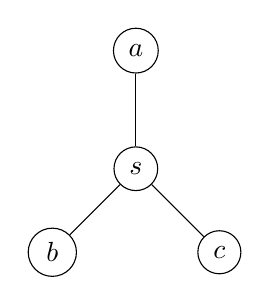
\begin{tikzpicture}[node distance={15mm},main/.style = {draw, circle}]
            \node[main] (s) {$s$};
            \node[main] (a) [above of=s] {$a$};
            \node[main] (b) [below left of=s] {$b$};
            \node[main] (c) [below right of=s] {$c$};
            \draw (s) -- (a);
            \draw (s) -- (b);
            \draw (s) -- (c);
        \end{tikzpicture}
    \end{center}
    We define an event structure where
    $\mathcal{E} = \s{a,b,c,i}$.
    We let $a,b,c$ to represent the events of sending
    a packet from $a$,$b$ and $c$ to $s$ respectively.
    Let $i$ indicate the event of the forwarding of
    an arbitrary packet from $s$ to $a$ (this may coming
    from either $b$ or $c$).
    We consider an empty conflict relation and enabling
    relation the least one for which we have:
    \begin{align*}
        \e \vdash b, \e \vdash c,
        \s{b} \vdash i, \s{c} \vdash i
    \end{align*}
    So, the configuration $\sigma = \s{b,c,i}$ is a
    counterexample since $i$ is happened while $a$
    has not been happened yet.
    Regarding this event structure we have:
    \begin{align*}
        \f{E(\e,b)}      & = M(\e,b) \wedge Con(\e) = M(\e,b)                                   \\
        \f{E(\s{b},c)}   & = (M(\s{b},c) \vee E(\e,c)) \wedge Con(\s{b})                        \\
                         & = M(\s{b},c) \vee E(\e,c)                                            \\
        \f{E(\e,c)}      & = M(\e,c) \wedge Con(\e)  = M(\e,c)                                  \\
        \f{E(\s{b,c},i)} & = (M(\s{b,c},i) \vee E(\s{b},i) \vee E(\s{c},i))
        \wedge Con(\s{b,c})                                                                     \\
        \f{E(\s{b},i)}   & = (M(\s{b},i) \vee E(\e,i))\wedge Con(\s{b})                         \\
                         & = M(\s{b},i) \vee E(\e,i)                                            \\
        \f{E(\s{c},i)}   & = (M(\s{c},i) \vee E(\e,i))\wedge Con(\s{c})                         \\
                         & = M(\s{c},i) \vee E(\e,i)                                            \\
        \f{M(\e,b)}      & = Min(\e,b) \wedge Con(\e) = Min(\e,b)                               \\
        \f{M(\e,c)}      & = Min(\e,c) \wedge Con(\e) = Min(\e,c)                               \\
        \f{M(\s{b},i)}   & = Min(\s{b},i) \wedge Con(\s{b}) = Min(\s{b},i)                      \\
        \f{M(\s{c},i)}   & = Min(\s{c},i) \wedge Con(\s{c}) = Min(\s{c},i)                      \\
        Min(\e,b)        & = \neg (M(\s{i},b) \vee M(\s{a},b) \vee M(\s{c},b) \vee M(\s{i,a},b) \\
                         & \vee M(\s{i,c},b) \vee M(\s{a,c},b) \vee M(\s{a,c,i},b))             \\
        Min(\e,c)        & = \neg (M(\s{i},c) \vee M(\s{a},c) \vee M(\s{c},c) \vee M(\s{i,a},c) \\
                         & \vee M(\s{i,c},c) \vee M(\s{a,c},c) \vee M(\s{a,c,i},c))             \\
        Min(\s{b},i)     & = \neg (M(\e,i)\vee M(\s{a,b},i) \vee M(\s{c,b},i)
        \vee M(\s{a,b,c},i))                                                                    \\
        Min(\s{c},i)     & = \neg (M(\e,i)\vee M(\s{a,c},i) \vee M(\s{b,c},i)
        \vee M(\s{a,b,c},i))                                                                    \\
    \end{align*}
    Let $\pi = b,c,i$ be a permutation of $\sigma$, we have:
    \begin{align*}
        \varphi_{\pi} & =
        E(\e,b) \wedge E(\s{b},c) \wedge E(\s{b,c},i)
        \wedge Con(\sigma)                            \\
        \varphi       & = \varphi_{\pi} \vee \varphi'
    \end{align*}
    This time, we can declare $M(\s{a,b},i) = \F$ as a cause of $\varphi$.
    Let $(M(\s{c},i),\F,\T)$ be the witness.
    We need to verify the following conditions:
    \begin{itemize}
        \item AC1:  $\m \vDash M(\s{a,b},i) = \F \wedge \varphi$
        \item AC2(a): $\m\vDash [M(\s{a,b},i)\la \T,M(\s{c},i)\leftarrow \F] \neg \varphi$
        \item AC2(b): $\m \vDash [\vec W' \la \vec w', \vec Z' \la \vec z^* ]\varphi$
              for all subsets
              $\vec W'$ of $\vec W$ and $\vec Z'$ of $\vec Z$.
    \end{itemize}
    Regarding the definition of functions for the $M_{k,i}$ variables,
    each variable $M_{k,i}$ is constantly false (until being intervened)
    if $s_k \not \vdash_{min} i$.
    Thus we have:
    \begin{align*}
        M & \vDash E(\e, b) = \T       \\
        M & \vDash E(\e, c) = \T       \\
        M & \vDash E(\s{b},c) = \T     \\
        M & \vDash E(\s{b},i ) = \T    \\
        M & \vDash E(\s{c},i ) = \T    \\
        M & \vDash E(\s{b,c},i) = \T   \\
        M & \vDash Con(\s{b,c,i}) = \T \\
        M & \vDash \varphi_{\pi}       \\
        M & \vDash \varphi
    \end{align*}
    Now we set $M(\s{a,b},i)$ to true and $M(\s{c},i)$ to false.
    Setting $M(\s{c},i)$ to false causes $E(\s{c},i)$ to be false.
    Setting $M(\s{a,b},i)$ to false causes $Min(\s{b},i)$ to false
    and subsequently $M(\s{b},i)$ and $E(\s{b},i)$ become false.
    Now, since all three terms in the first conjunction of the $\f{E(\s{b,c},i)}$
    so $E(\s{b,c},i)$ becomes false and this results in $\varphi$ become false.
    To verify AC2(b), assume that we have set $M(\s{c},i)$ to false.
    This makes $E(\s{c},i)$ false.
    But, since $\f{E(\s{b,c},i)}$ includes the term
    $E(\s{b},i) \vee E(\s{c},i)$ and $E(\s{b},i)$ is true, regardless
    of the value of $M(\s{c},i)$, thus changing $M(\s{c},i)$ has
    no effect on $(E(\s{b,c},i))$ and thus does not affect
    the value of $\varphi$, so AC2(b) is satisfied.
\end{example}
